\begin{frame}{\textbf{Scholarfy: usage}}

\begin{figure}
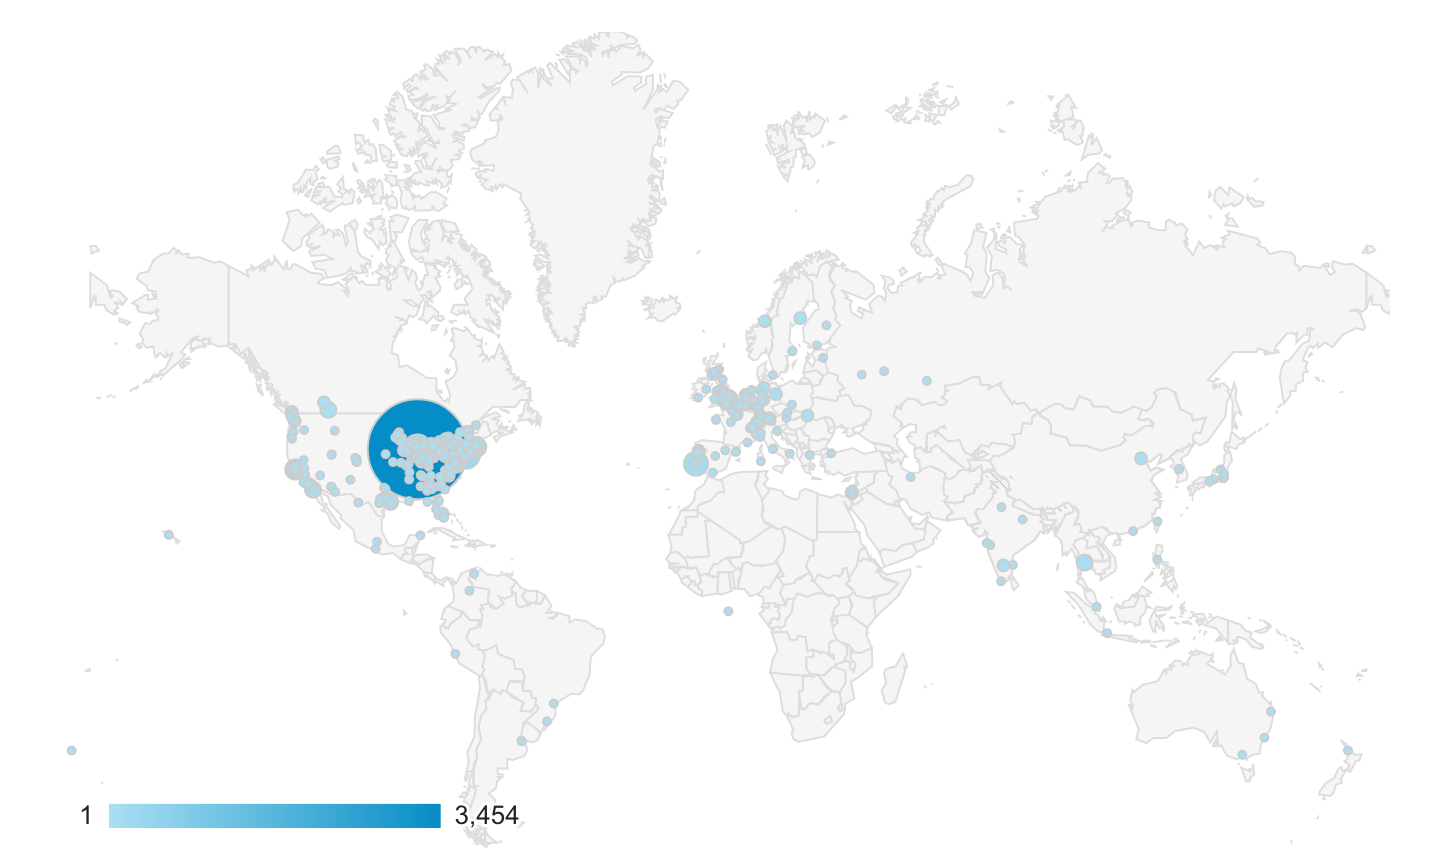
\includegraphics[width=2.5in]{images/scholarfy_map}\\
\end{figure}

\begin{center}
"@KordingLab I joined twitter specifically to thank you for this site. Great job!"
\end{center}

\end{frame}


\begin{frame}{\textbf{Discussion}}

\begin{itemize}
\item Scalability - LSA is still a batch, large scale nearest neighbor (project with Knowledge lab)
\item Suggestion - science concierge tends to do better when user like one topic
\end{itemize}

\end{frame}


\begin{frame}{\textbf{Applying Scholarfy to review process: COSYNE}}

\begin{center}
\href{http://cosyne.scienceofscience.org/}{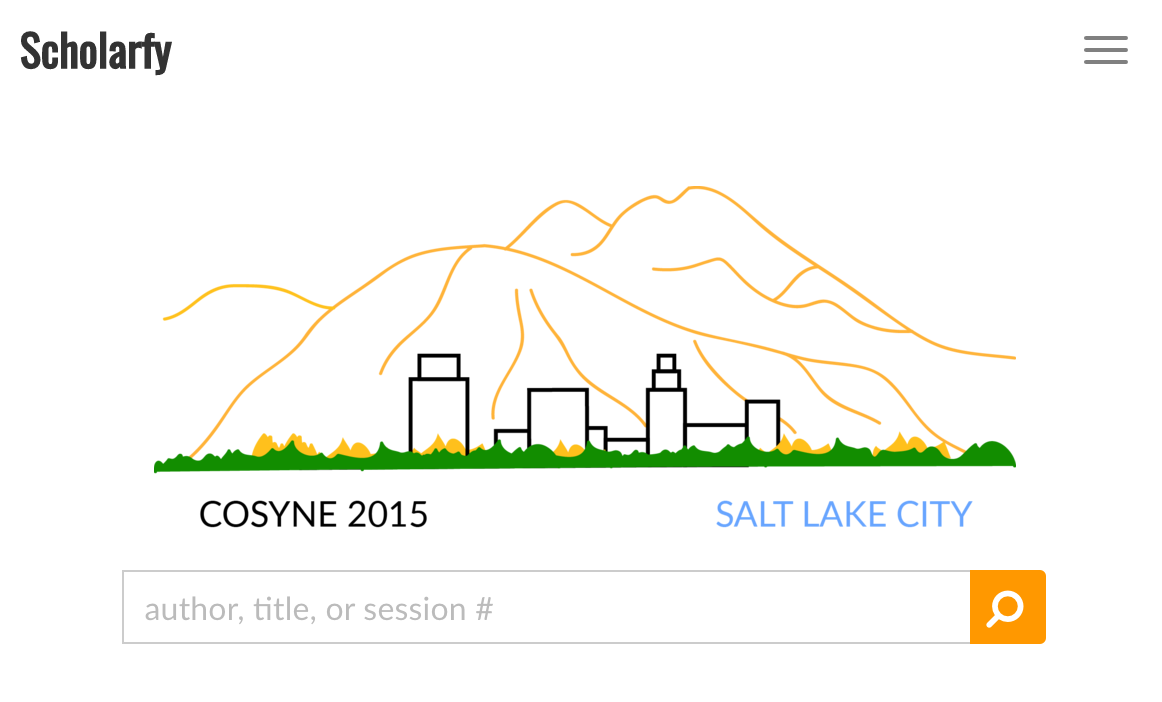
\includegraphics[width=2.0in]{images/cosyne}}
\end{center}

\begin{itemize}
\item Let reviewers choose preference papers from last year
\item Match paper to reviewers based on preferences
\end{itemize}

\end{frame}



\begin{frame}{\textbf{Acknowledgement}}

For great mentorship and suggestion
\begin{itemize}
\item Daniel Acuna
\item Konrad Kording
\end{itemize}

For great friendship and Github support
\begin{itemize}
\item Tulakan Ruangrong
\end{itemize}

\begin{center}

\includegraphics[width=1.5in]{images/octobiwan}
\end{center}

\end{frame}


\begin{frame}{\textbf{Github projects}}

\begin{itemize}
\item \href{https://github.com/titipata/science\_concierge}{\textcolor{gray}{\texttt{titipata/science\_concierge}}}
\item \href{https://github.com/tribbloid/spookystuff}{\textcolor{gray}{\texttt{tribbloid/spookystuff}}}
\end{itemize}

\begin{center}

\includegraphics[width=1.5in]{images/octobiwan}
\end{center}

\end{frame}


\begin{frame}

\begin{center}
\textbf{Q/A}
\end{center}

\begin{center}

\includegraphics[width=3.5in]{images/cover_back}
\end{center}

\end{frame}
